\documentclass[11pt]{article}
\usepackage[margin=0.75in]{geometry}
\usepackage{graphicx}
\usepackage{siunitx}
\usepackage{amsmath}
\usepackage{float}
\usepackage{caption}
\usepackage{booktabs}
\usepackage{circuitikz}
\usepackage{url}


\title{Exploring Pulse Waves in a Coax Cable}
\author{Jason Jain, Hannah Speckman, Owen Schlimgen \\
        Oregon State University, Department of Physics \\
        Electronics Laboratory}
\date{\today}

\graphicspath{{output/}}

\begin{document}

\maketitle

\begin{abstract}
  Coax cables transmit voltage waves at high fractions of light speed and are ubiquitous in modern communications. We send a pulsed wave through a $\qty{156}{\meter}$ long RG-58 coax cable, observe the waveform with an oscilloscope, and calculate the wave speed to be $\qty{1.97e8}{\meter / \s}$, matching the spec sheet value of 66\% of the speed of light to within 1.5\%. To simulate a boundary, we use a splitter with a terminating resistor connected to a second oscilloscope channel and measure the amplitudes of the incident, reflected, and transmitted pulses to determine the reflection and transmission coefficients. We observe the expected behavior across a range of terminating resistances, and find that a lightly damped model incorporating cable resistance better accounts for amplitude losses at high terminating impedances.
\end{abstract}

\section{Introduction}\label{sec:introduction}

Coax cables are foundational to modern communications, used for transmitting internet, telephone, and television signals worldwide. A coax cable consists of four layers---a center conductor, a dielectric insulator, an outer conducting shield, and a protective jacket---and can be modeled as a distributed transmission line with resistance $R$, inductance $L$, and capacitance $C$ per unit length~\cite{gfgcoax}.

We develop and test a model for wave propagation, reflection, and transmission in such a cable. We set up a $\qty{156}{\meter}$ long RG-58 coax cable driven by a function generator; oscilloscope channels are connected at the near and far ends to measure incident, reflected, and transmitted pulses. In the first experiment we measure the wave propagation speed; in the second we measure reflection and transmission coefficients for a range of terminating resistances and compare to theoretical predictions, including a lightly damped correction for cable losses.



\begin{figure}[htbp]
  \centering

  \begin{circuitikz}[american]
    % Source and scope CH1 at near end
    \draw
    (0,0) to[sV,l=$V_{\text{in}}$] (0,3)
    to[short] (2,3)
    (2,3) to[short] (3,3)
    % Long coax segment (modeled as a generic two-port)
    to[generic,l=$L \approx \qty{156}{\meter}$] (6,3)
    % Termination and scope CH2 at far end
    to[short] (9,3)
    (9,3) to[R,l=$R_{\text{term}}$] (9,0)
    to[short] (0,0);
    \draw (2,0)
    to[oscope, l_=$CH1$] ++(0, 3);
    \draw (7,0)
    to[oscope, l=$CH2$] ++(0, 3);
  \end{circuitikz}

  \caption{Experimental setup for the coax cable lab. A pulsed voltage $V_{\text{in}}$ from a function generator is launched into a \qty{156}{\meter} RG-58 coax cable (characteristic impedance $Z_0 \approx \qty{53.5}{\ohm}$). Channel~1 (CH1) monitors the input end, capturing both the outgoing incident pulse and the pulse reflected from the far end. Channel~2 (CH2) monitors the transmitted pulse across a variable terminating resistor $R_{\text{term}}$, which simulates a wave crossing into a medium of different impedance. Varying $R_{\text{term}}$ from below to above $Z_0$ sweeps the reflection coefficient from negative through zero to positive, providing a clean test of the transmission-line boundary model.}
  \label{fig:coax_setup}
\end{figure}


\section{Theory}\label{sec:theory}

We model a lightly damped traveling wave $\psi(x,t)$ with Eq.~\eqref{wave}, where $\Gamma$ is the damping coefficient, $A$ is the amplitude, $\phi$ is the phase, and the wave speed is $v=\omega/k$ \cite{georgi}.

\begin{equation}
  \label{wave}
  \psi(x,t) = A\,e^{-\Gamma x/2v}\cos(\omega t \pm kx + \phi)
\end{equation}

At a boundary between two media, an incident wave $\psi_I$ (amplitude $A$) splits into a reflected wave $\psi_R$ (amplitude $B$) and a transmitted wave $\psi_T$ (amplitude $C$). Continuity of displacement and material velocity at the boundary requires

\begin{equation}
  \label{boundary_cond}
  A+B=C, \quad (A-B)\,k_1 = C\,k_2
\end{equation}

The reflection and transmission coefficients follow from Eq.~\eqref{boundary_cond} and the impedance $z$ of each medium \cite{georgi}:

\begin{equation}
  \label{coeff}
  R\equiv \frac{B}{A}= \frac{z_2-z_1}{z_2 + z_1}, \quad T\equiv \frac{C}{A}= \frac{2z_1}{z_2 + z_1}
\end{equation}

Notice that $T = 1 + R$ for all cases. Substituting values our cable with characteristic impedance $Z_0=\qty{53.5}{\ohm}$ (from the data sheet) and terminating resistance $R_\mathrm{term}$ acting as $z_2$:

\begin{equation}
  \label{th_coeff}
  R_\mathrm{th}= \frac{R_\mathrm{term}-Z_0}{R_\mathrm{term} + Z_0}, \quad T_\mathrm{th}= \frac{2Z_0}{R_\mathrm{term} + Z_0}
\end{equation}

For a more accurate prediction, we can take damping into account. Using $v=1/\sqrt{L_0C_0}$, the damping factor in Eq.~\eqref{wave} yields an amplitude decay $e^{-\Gamma L/2v}$ over cable length $L$. The underdamped correction is valid for $R_0 \ll Z_0$ and accounts for resistive losses that the ideal model neglects.


\begin{equation}
  \label{damp_coeff}
  \frac{\Gamma}{2v}=\frac{R_0C_0 v}{2}
\end{equation}



\section{Results}\label{sec:results}


\begin{table}[H]
  \centering
  \caption{Reflection and transmission coefficients for a range of terminating resistances. $R = V_R/V_I$ and $T = V_T/V_I$ are computed from cursor-measured pulse heights. Reflection is negative for $R_\mathrm{term} < Z_0$, near zero at the matched condition $R_\mathrm{term} \approx Z_0$, and positive for $R_\mathrm{term} > Z_0$; transmission exceeds unity when $R > 0$, consistent with $T = 1+R$. Interpolating the $R \approx 0$ row gives an experimental cable impedance $Z_{0,\mathrm{exp}} = \qty{53.8}{\ohm}$. The last row is the open-circuit limit ($R_\mathrm{term} \to \infty$), corresponding to Figure~\ref{fig:pic1}.}
  \label{tab:data}
  \small
  \begin{tabular}{
      S[table-format=3.1]
      S[table-format=1.2]
      S[table-format=1.3]
      S[table-format=-1.3]
      S[table-format=-1.3]
      S[table-format=1.3]
    }
    \toprule
    {$R_{\mathrm{term}}$ (\unit{\ohm})} & {$V_{I}$ (\unit{V})} & {$V_{T}$ (\unit{V})} & {$V_{R}$ (\unit{V})} & {$R = V_{R}/V_{I}$} & {$T = V_{T}/V_{I}$} \\
    \midrule
    20.0                                & 1.48                 & 0.672                & -0.660               & -0.446              & 0.454               \\
    29.8                                & 1.50                 & 0.880                & -0.352               & -0.235              & 0.587               \\
    50.3                                & 1.48                 & 1.240                & -0.018               & -0.012              & 0.838               \\
    74.5                                & 1.50                 & 1.500                & 0.108                & 0.072               & 1.000               \\
    118.4                               & 1.50                 & 1.820                & 0.260                & 0.173               & 1.213               \\
    148.0                               & 1.40                 & 1.940                & 0.320                & 0.229               & 1.386               \\
    {$\infty$}                          & 1.54                 & 2.680                & 0.660                & 0.429               & 1.740               \\
    \bottomrule
  \end{tabular}
\end{table}


\subsection{Measuring Wave Speed}


\begin{figure}[H]
  \centering
  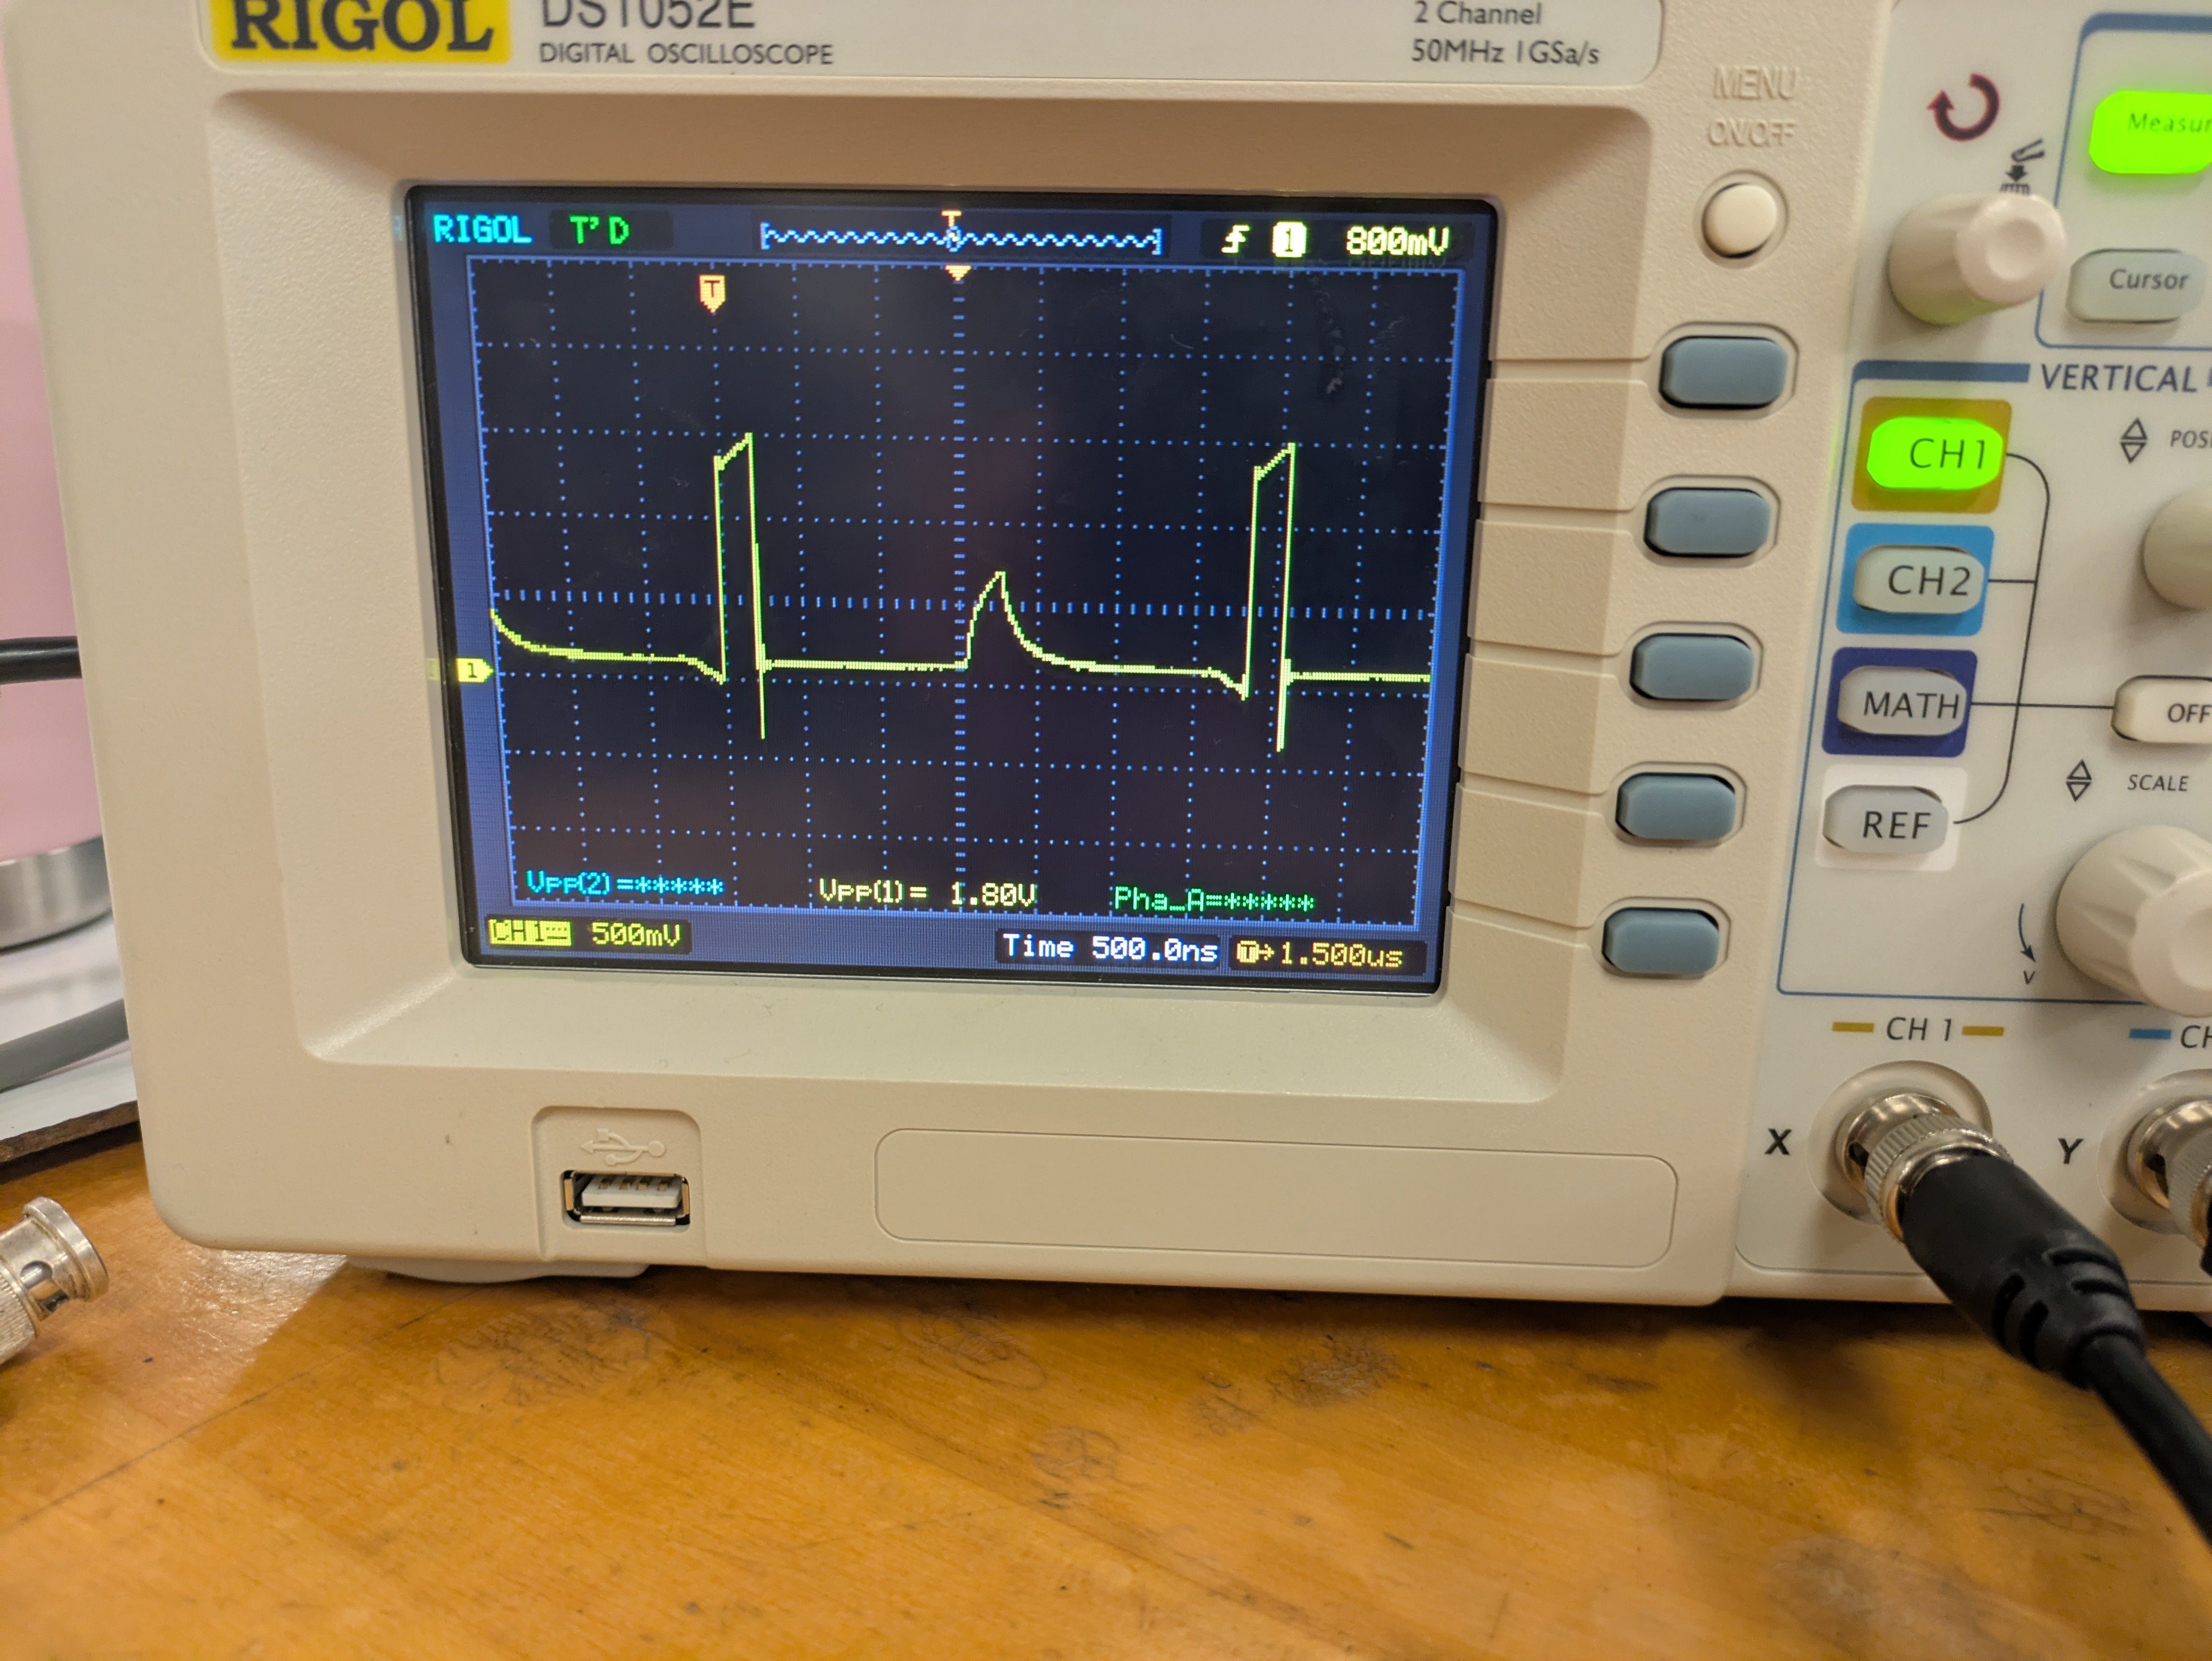
\includegraphics[width=0.5\columnwidth]{data/pic2.jpg}
  \caption{Oscilloscope trace showing the incident voltage pulse (\qty{1.86}{\volt}, first peak) and the pulse reflected from the open far end (second peak). Cursors measure the round-trip travel time $\Delta t = \qty{1.56}{\micro\s}$, from which the wave speed is calculated via Eq.~\eqref{wave_vel}.}
  \label{fig:pic1}
\end{figure}


To measure wave speed, we connected CH1 at the input end and left the far end open (no terminating resistor), capturing the outgoing pulse and the pulse returning after reflecting from the open end. A voltage pulse of height $\qty{1.86}{\volt}$ was launched into the cable, and using the oscilloscope cursors, we measured a round-trip time $\Delta t = \qty{1.56}{\micro\s}$; since the pulse travels $2l = \qty{312}{\meter}$ in that interval:

\begin{equation}
  \label{wave_vel}
  v=\frac{2l}{\Delta t}=0.657c=\qty{1.97e8}{\meter\per\second}
\end{equation}

This agrees with the data sheet specification of 66\% of $c$ to within 1.45\%. This is the phase velocity of the electromagnetic wave, not the drift velocity of the conduction electrons. The electrons' material velocity is far smaller: each electron oscillates only slightly to advance the disturbance to its neighbor, similar to sound propagating through air.


\subsection{Characterizing Reflection and Transmission}


\begin{figure}[H]
  \centering
  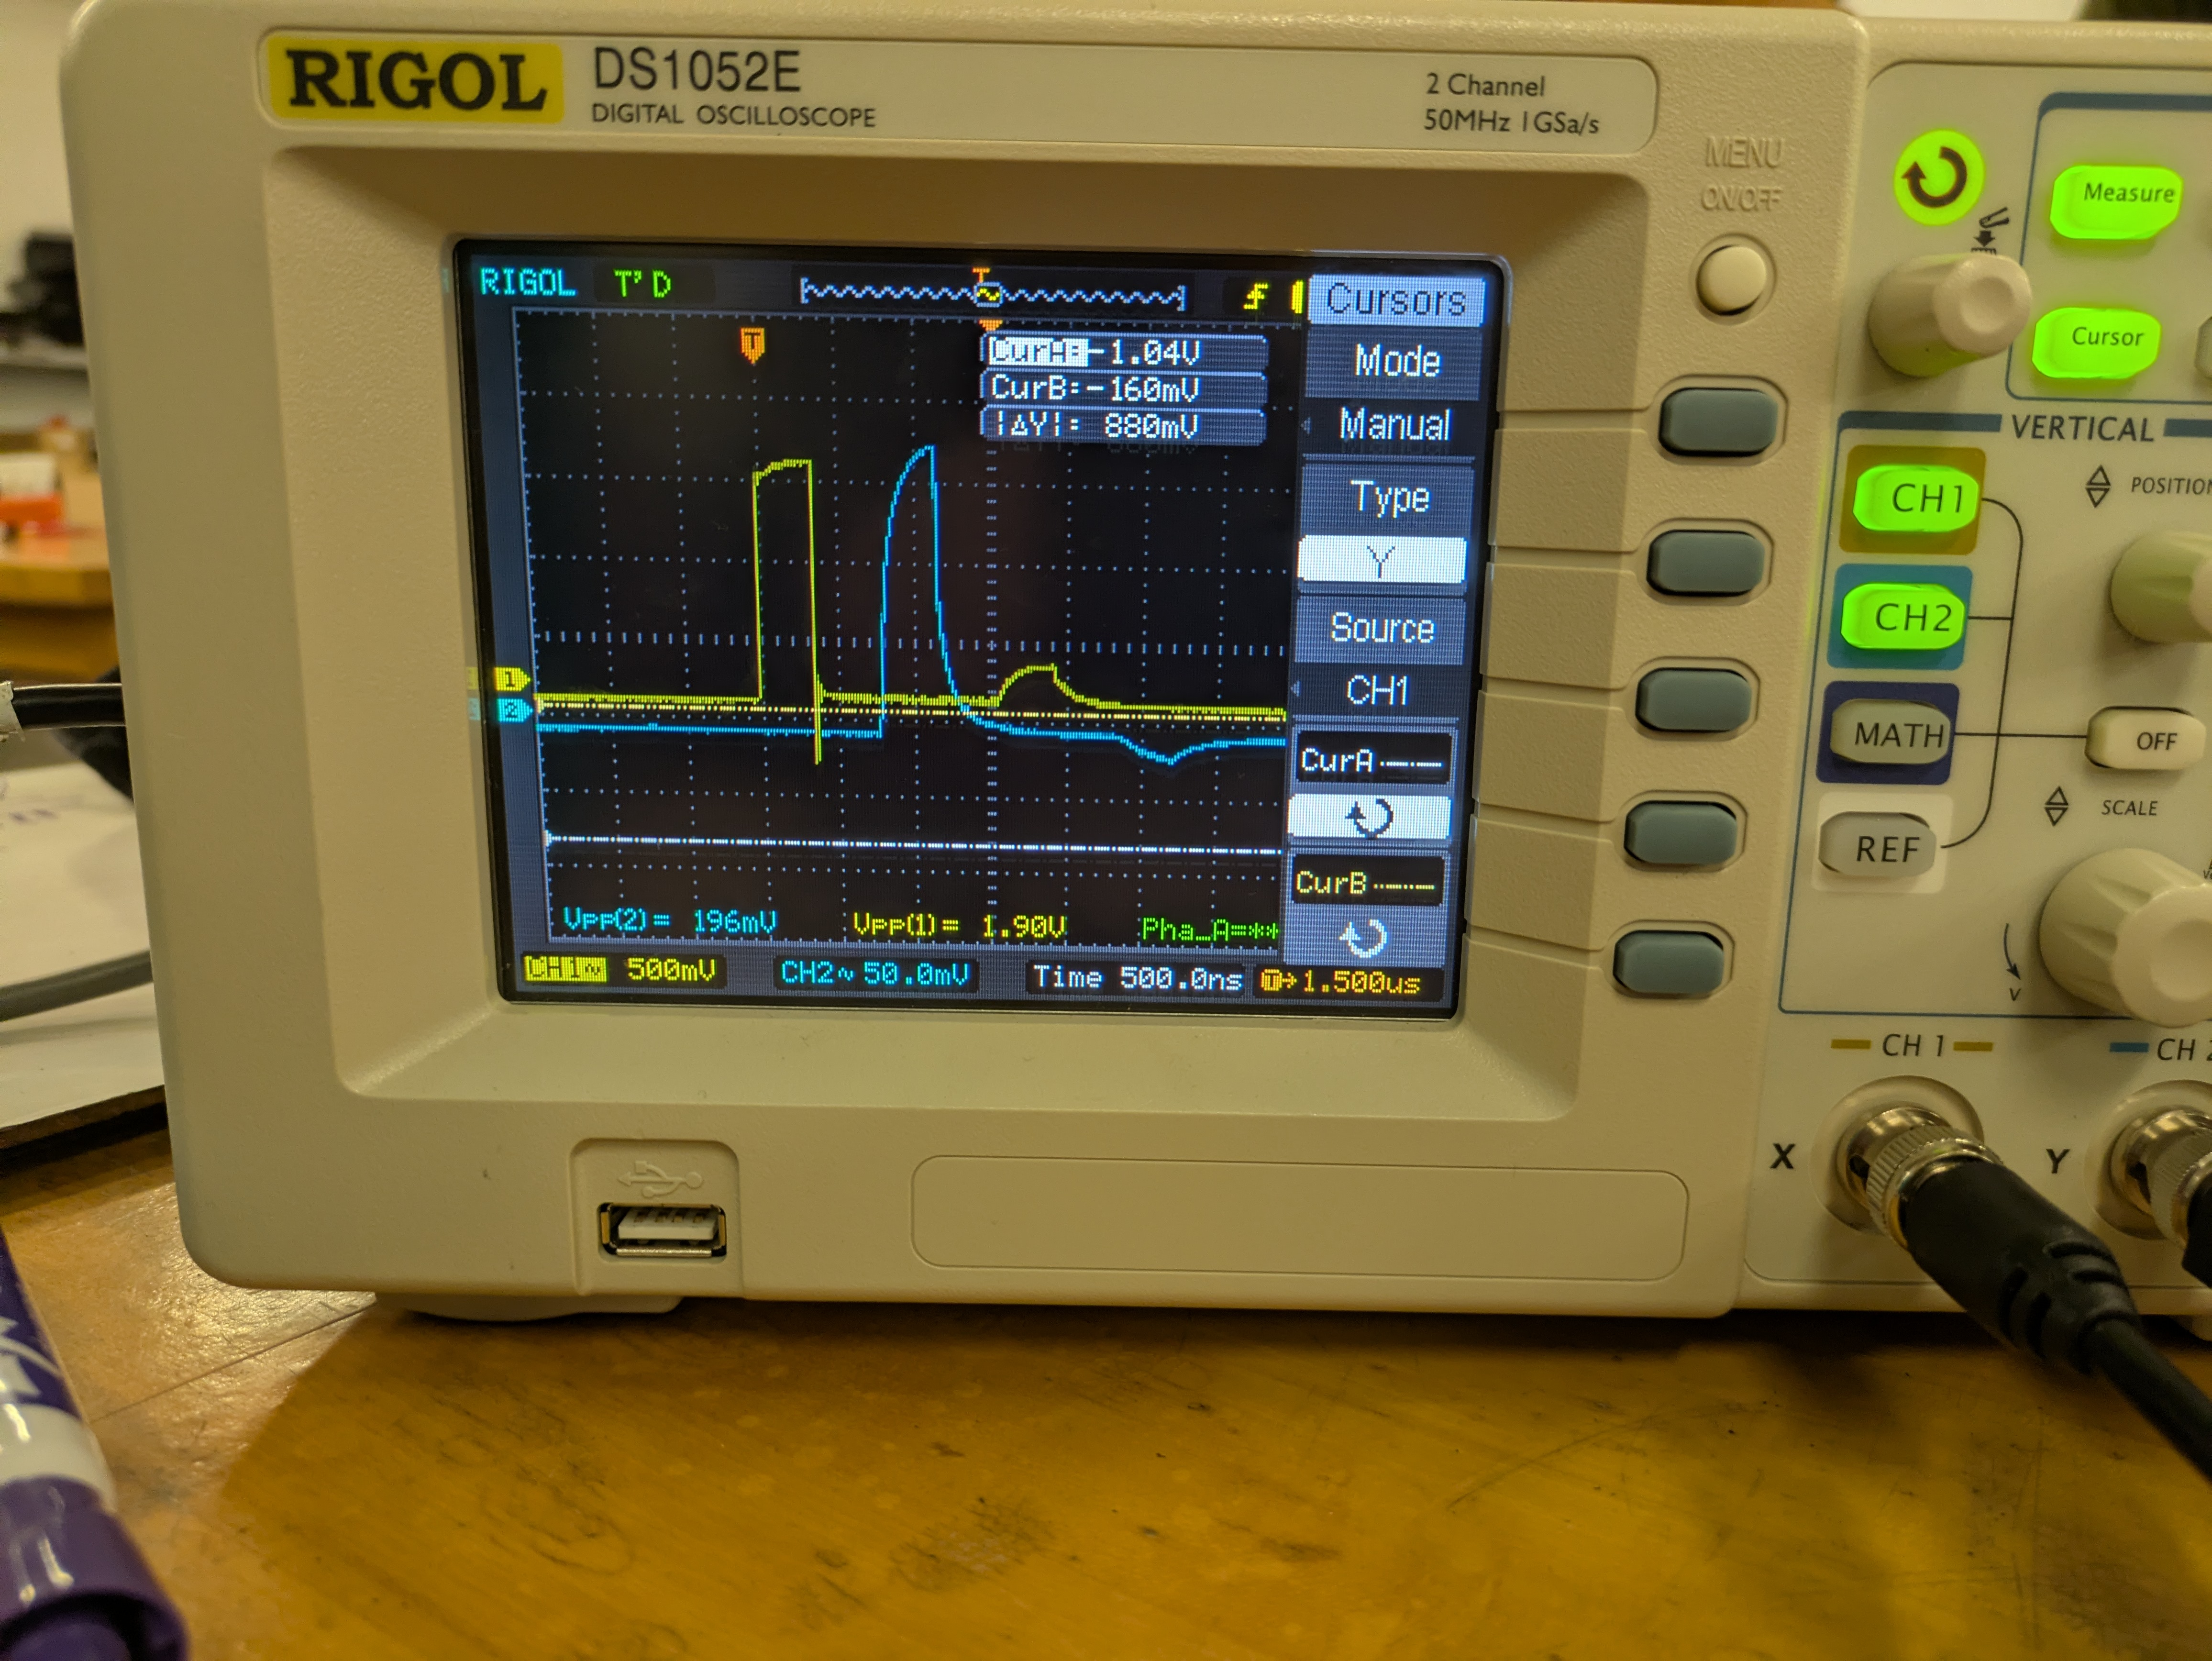
\includegraphics[width=0.5\columnwidth]{data/pic4.jpg}
  \caption{Oscilloscope trace with a terminating resistor attached. The first yellow peak is the incident pulse (\qty{1.86}{\volt}); the second yellow peak is the reflection at CH1; the blue peak is the transmission at CH2 across $R_\mathrm{term}$. Pulse heights are read with cursors. The two channels are scaled independently for clarity.}
  \label{fig:pic2}
\end{figure}


In the second experiment, we attached terminating resistors ranging from $20$ to $\qty{150}{\ohm}$ to the far end and connected CH2 across each resistor (Figure~\ref{fig:coax_setup}). For each value of $R_\mathrm{term}$ we used cursors to read the incident ($V_I$), reflected ($V_R$), and transmitted ($V_T$) pulse heights, giving the measured coefficients $R = V_R/V_I$ and $T = V_T/V_I$ listed in Table~\ref{tab:data}.



\begin{figure}[H]
  \centering
  \includegraphics[width=0.65\columnwidth]{wave_propagation.png}
  \caption{Reflection coefficient $R$ and transmission coefficient $T$ vs.\ terminating resistance $R_{\mathrm{term}}$. Points are measured values from Table~\ref{tab:data}; solid curves are the undamped model from Eq.~\eqref{th_coeff} with $Z_0 = \qty{53.5}{\ohm}$. The cable impedance is read directly from the data by interpolating where $R = 0$, giving $Z_{0,\mathrm{exp}} = \qty{53.8}{\ohm}$ (within 0.6\% of the data sheet value). At higher $R_\mathrm{term}$, measured amplitudes fall systematically below the ideal curves, suggesting an energy-loss mechanism not captured by the undamped model.}
  \label{fig:wave_propagation}
\end{figure}


The undamped model fits well at low to moderate resistances but overestimates amplitudes at high $R_\mathrm{term}$ (Figure~\ref{fig:wave_propagation}). This systematic shortfall points to resistive energy loss in the cable. Incorporating the damping factor from Eq.~\eqref{damp_coeff} with $C_0 = \qty{100}{\pico\farad\per\meter}$ and $v = \qty{1.97e8}{\meter\per\second}$ gives $\Gamma/2v = \qty{3.86e-4}{\per\meter}$, so a pulse traversing the cable is attenuated by $e^{-\Gamma L/2v} = 0.89$---an 11\% amplitude reduction. The cable's total resistance $R_0 L = \qty{0.0392}{\ohm\per\meter} \times \qty{156}{\meter} = \qty{6.1}{\ohm}$ is small compared to $Z_0 = \qty{53.5}{\ohm}$, confirming the light-damping approximation is appropriate.


\begin{figure}[H]
  \centering
  \includegraphics[width=0.65\columnwidth]{wave_propagation_damping.png}
  \caption{Same data as Figure~\ref{fig:wave_propagation} with the under correction added. Dashed curves include the attenuation factor $e^{-\Gamma L/2v}$ from Eq.~\eqref{damp_coeff} with $\Gamma/2v = \qty{3.86e-4}{\per\meter}$. The damped model reduces the systematic over-prediction at high $R_\mathrm{term}$, confirming that resistive loss in the cable is the primary source of the discrepancy seen in Figure~\ref{fig:wave_propagation}.}
  \label{fig:wave_propagation_damping}
\end{figure}

\section{Conclusions}\label{sec:conclusions}

We investigated pulse propagation in a \qty{156}{\meter} RG-58 coax cable, testing models for wave speed and for reflection and transmission at a resistive boundary. Setting up a $\qty{156}{\meter}$ long RG-58 coax cable with a two-channel oscilloscope, we observed the reflection and transmission of voltage pulses with varying terminating resistances. We found a wave speed of $\qty{1.97e8}{\meter\per\second}$, within 1.5\% of the data-sheet value of $0.66c$. Measured reflection and transmission coefficients follow our predicted trends, and we use our data to calculate an experimental $Z_0 = \qty{53.8}{\ohm}$, within 0.6\% of the data sheet value. Predicted coefficients overshoot for larger $R_\mathrm{term}$, so we offer a more accurate damping model with an 11\% attenuation factor, calculated from the cable's total resistance ($\qty{6.1}{\ohm}$). The damped model has better agreement with the data, but still has minor discrepancies from inefficiencies in the circuit and component tolerances. However, our model is still a powerful tool for capturing the basic physics of coax cables, and can be used for impedance-matching transmission and minimizing signal loss from reflection.

\newpage

\begin{thebibliography}{9}
  \bibitem{georgi}
  H. Georgi, The Physics of Waves. Addison Wesley Publishing Company, 1993.
  \bibitem{gfgcoax}
  GeeksforGeeks, ``What is Coaxial Cable?'' \url{https://www.geeksforgeeks.org/computer-networks/what-is-coaxial-cable/}
  \bibitem{copilot}
  GitHub Copilot GPT-5.1, AI-powered code completion tool by GitHub. Used for assistance with Python code development and \LaTeX\ formatting. \url{https://github.com/features/copilot}
\end{thebibliography}

\section*{Addendum}
The native language of the author(s) is English.

\end{document}